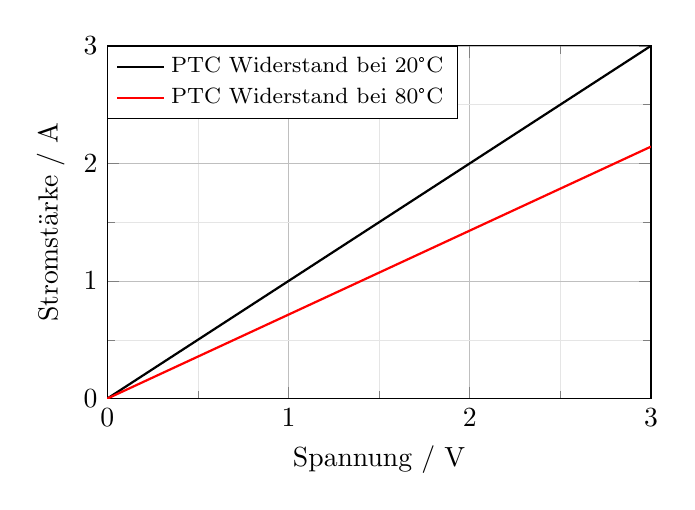
\begin{tikzpicture}
    \begin{axis}[
            xlabel={Spannung / V},
            ylabel={Stromstärke / A},
            xmin=0, xmax=3,
            ymin=0, ymax=3,
            xtick={0,1,2,3},
            ytick={0,1,2,3},
            minor x tick num=1,
            minor y tick num=1,
            grid=both,
            major grid style={line width=.2pt,draw=gray!50},
            minor grid style={line width=.1pt,draw=gray!20},
            legend style={font=\footnotesize, at={(0,1)}, anchor=north west},
            width=0.7\textwidth, % Adjust the width of the plot
            height=0.5\textwidth % Adjust the height of the plot
        ]

        % Temperaturunabhängiger Widerstand (Steigung 1)
        \addplot[
            color=black,
            mark=none,
            thick,
        ] coordinates {
                (0,0)(3,3)
            };
        \addlegendentry{PTC Widerstand bei 20°C}

        % Temperaturabhängiger Widerstand (Steigung 1/1.4)
        \addplot[
            color=red,
            mark=none,
            thick,
        ] coordinates {
                (0,0)(3,3/1.4)
            };
        \addlegendentry{PTC Widerstand bei 80°C}

    \end{axis}
\end{tikzpicture}